% !TEX root = ../thesis.tex
\chapter{Approach}
\label{ch:approach}
% **************************** Define Graphics Path **************************
\ifpdf
\graphicspath{{Chapter3/Figs/Raster/}{Chapter3/Figs/PDF/}{Chapter3/Figs/}}
\else
\graphicspath{{Chapter3/Figs/Vector/}{Chapter3/Figs/}}
\fi

\section{Introduction}
\label{sec:approachIntro}
Despite the importance of crowd monitoring in mass gathering events, the literature review in the previous chapter is able to identify several gaps in the research, especially in crowd modelling. Most state-of-art crowd monitoring techniques do not incorporate a typology to distinguish different types of crowd. In other words, no explicit type of crowd is defined in those approaches.

say something more about crowd modelling

conclude with the need of a crowd monitoring framework

\section{An Overview of the Crowd Monitoring Framework}

The literature review in Chapter \ref{ch:litReview} has summarised that most of the state-of-art crowd monitoring approaches are focusing on using computer vision to automate the analysis of CCTV system. The literature review has also noted several limitations of the computer vision technique, such as the effect of obstacles and low lighting condition. With the rapid development of mobile computing and the increasing popularity of mobile devices, mobile sensing seems to be a more potential technique to collect contextual data for crowd monitoring. Information about the context are obtained from a variety of sensors integrated in mobile phones and wearable devices, for example GPS receivers and accelerometers. Apart from those ``hard sensors'', the literature review also highlights that another type of information source known as the ``soft sensor'' can be used to monitor the peace of a crowd, which is the social media. The use of social media analysis for crowd monitoring has been introduced in a related work by \citet{DelirHaghighi2013}. It has the great advantage of feasibility as it only relies on the software and no additional hardware is required to be installed. Despite this strength, our literature review shows that very limited works have been done to utilize social media to support emergency management.

Secondly, another finding from the literature review is that emotions are one of the key factors that form and motivate collective behaviours, which in our context are the crowd behaviours. Hence, it is essential for a crowd monitoring approach to consider the influence of emotions in the crowd. Although human emotion is an abstract concept and very difficult to measure with ``hard sensors'', it is very possible to capture the emotion of a person from the verbal expressions, such as writing or voice. This is where social media further proves its advantage over the ``hard sensors''. By applying analysis on the social media, we can capture the emotions in a crowd, thus enabling the inference of the crowd's condition. For that reason, in this project, we would like to propose a crowd monitoring framework that employs the emotion analysis of social media to support emergency management in mass gatherings. 

Finally, our literature review also reveals another gap in the research that is the lack of a crowd model that can distinguish different crowd types. Most existing crowd monitoring techniques do not base on any model thus making it difficult to identify exactly what crowd type is happening without the interpretation of human. By exploring broader into other disciplines, our literature review is able to point out several notable works on crowd modelling and classification in the police literature and public safely science. Among those works, Berlonghi's wowrk stands out as the most commonly adopted model by the emergency management bureaus worldwide. Our proposed crowd monitoring framework is established on the Berlonghi's model which consists of eleven different crowd types. Yet, a systematic approach to classify one crowd into those types is challenging because Berlonghi's model only describes the crowd types and there is no attribute defined in the existing model. Therefore, in our framework, we would like to propose a mapping model that links the emotion model with crowd model, enabling the crowd type classification by fuzzy logic.


In conclusion, the proposed framework addresses the gaps that are identified in the previous chapters by: 
\begin{inparaenum}[i)]
\item incorporating social media as the information source for context data;
\item capturing the emotions of a crowd by analysing the context data;
\item identifying the type of a crowd by applying fuzzy inference to the crowd emotions
\end{inparaenum}.

\begin{figure}[htbp!] 
\centering    
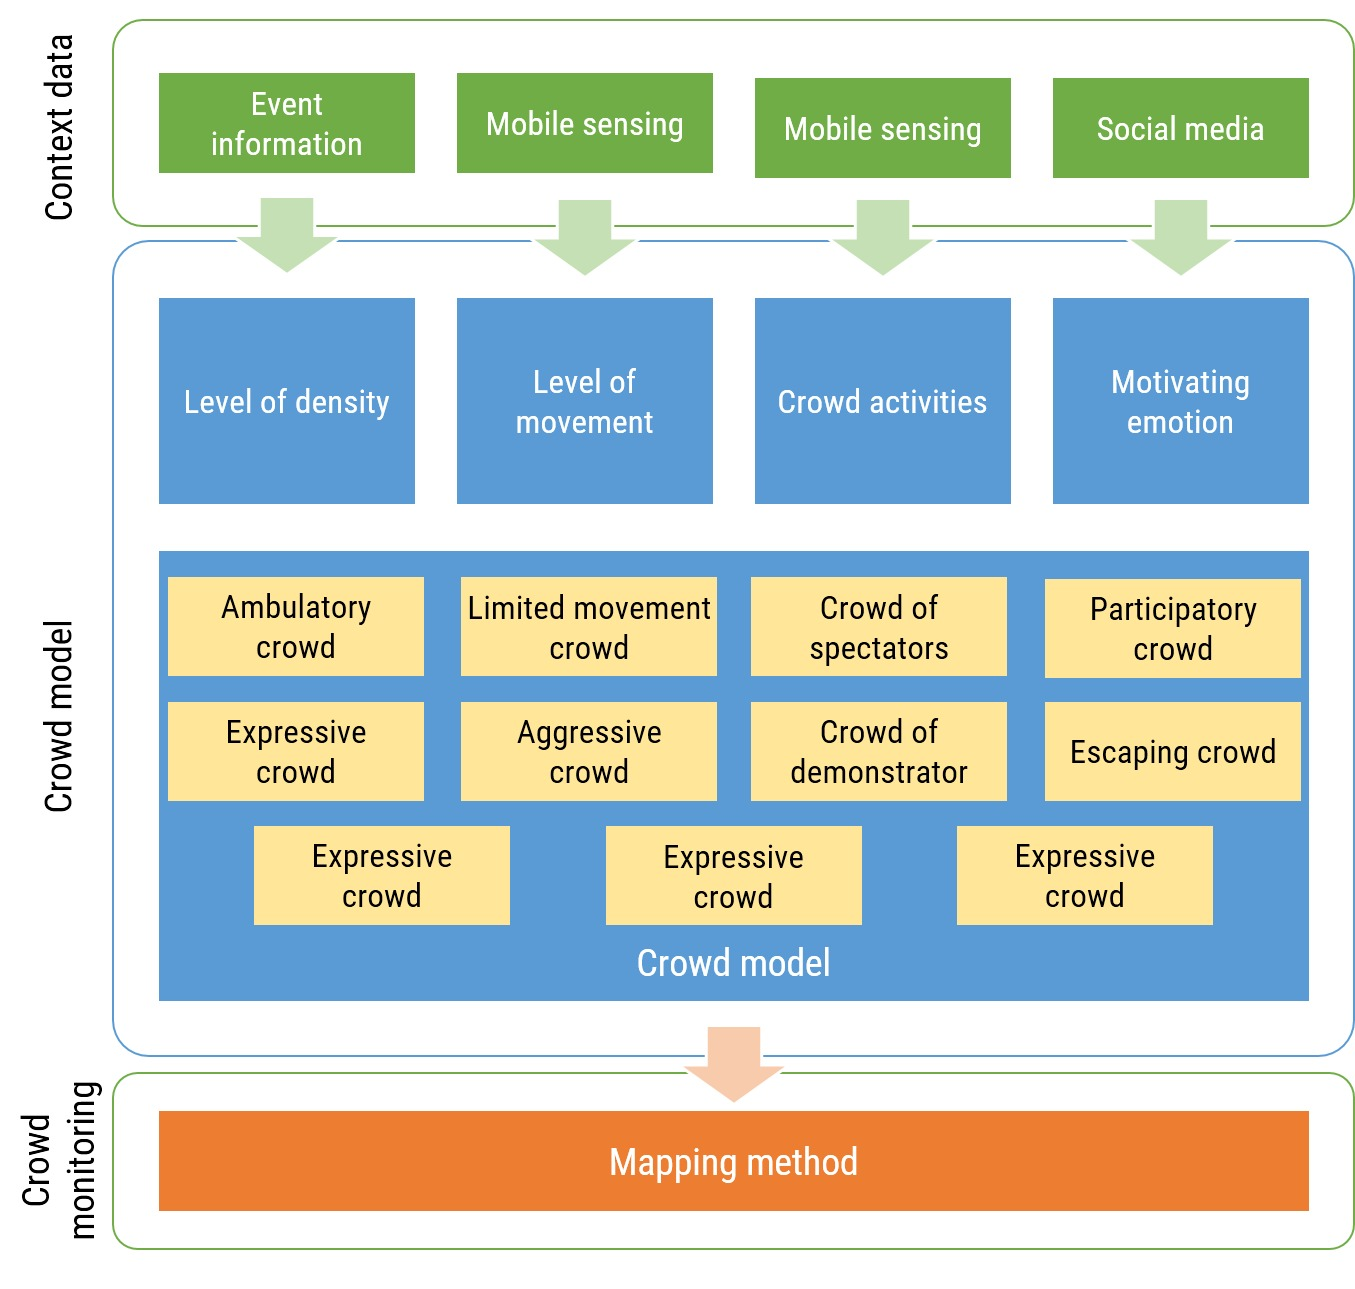
\includegraphics[width=1.0\textwidth]{FrameworkOverview}
\caption{An overview of the crowd monitoring framework using emotion analysis of social media}
\label{fig:frameworkOverview}
\end{figure}

As can be seen in Figure \ref{fig:frameworkOverview}, the framework consists of from following components:
\begin{inparaenum}[i)]
\item Emotion analysis;
\item Emotion model;
\item Crowd model;
\item Emotion - Crowd type mapping model;
\item Rule based reasoning
\end{inparaenum}. Each component will be discussed further in the sections below.

\section{Context data}
Social media is the generic term referring to a wide range of Internet based tools that enable user to create and share information. These tools include social network services such as Facebook and Twitter, Internet forums and channels. Among these tools, Twitter is the most common social media used in researches because of its large volume of users and its public API making the data highly accessible.

\section{Emotion Model}

We use Plutchik model

\section{Emotion Analysis of Social Media}

We can detect the dominating emotion from a tweet using a bag of word approach.

We then apply histogram with a specific time interval to measure the frequency of each emotion during that time frame.

\section{Crowd Model}

We use Berlonghi model

\section{Emotion - Crowd Type Mapping Model}

Table \ref{table:mappingEmotionCrowdType} presents our proposal for the mapping between each crowd type and eight basic emotions.
\begin{table}
\caption{Mapping between crowd types and emotions}
\label{table:mappingEmotionCrowdType}
\begin{tabular}{|p{2cm}|p{1.2cm}|p{1.2cm}|p{1.2cm}|p{1.2cm}|p{1.2cm}|p{1.2cm}|p{1.2cm}|p{1.2cm}|}
\hline
\textbf{Crowd type}	& \textbf{Anger}	& \textbf{Anticipation}	& \textbf{Joy} 	& \textbf{Trust}	& \textbf{Fear}	& \textbf{Surprise}	& \textbf{Sadness}	& \textbf{Disgust}	\\
\hline
Ambulatory			& low 				& medium				& medium		& medium			& low 			& low 				& medium			& low 		\\
\hline
Limited movement	& medium			& medium				& low 			& low 				& low 			& low 				& medium			& medium	\\
\hline
Spectator			& low 				& medium				& medium		& medium 			& low 			& medium			& low 				& low 		\\
\hline
Participatory		& low 				& medium				& medium		& medium			& low 			& low 				& low 				& low 		\\
\hline
Aggressive			& medium			& low 					& low 			& low 				& low 			& low 				& low 				& medium	\\
\hline
Demonstrator		& medium			& low 					& low 			& low 				& low 			& low 				& medium			& medium	\\
\hline
Escaping			& low 				& low 					& low 			& low 				& medium		& medium			& low 				& low 		\\
\hline
Dense				& medium			& low 					& low 			& low 				& medium		& medium			& low 				& medium	\\
\hline
Rushing				& medium			& low 					& low 			& low 				& low 			& low 				& low 				& medium	\\
\hline
Violent				& medium			& low 					& low 			& low 				& low 			& low 				& low 				& medium	\\
\hline
\end{tabular}
\end{table}

\section{Rule Based Reasoning}

\subsection{Fuzzifier}
We convert the numerical values of the frequency of appearance of an emotion into linguistic label: low, medium and high by applying following rules

if the value is below the low threshold of that emotion then the label is low
if the value is above the low threshold and below the high threshold then the label is medium
if the value is above the high threshold then the label is high

\subsection{Rule Repository}

list 11 rules here for 11 crowd types

\subsection{Inference Engine}

Fuzzy rule here and the mathematical formula here

\subsection{Output Processor}

the output is a vector of each crowd and its weight

\section{Conclusion}